\newpage

\section{Introduction}

The Anick part of the BERGMAN package \footnote{those are interested,
there is another anick C++ implementation whose source files are accessible
by anonymous ftp on the \tt{ftp://ftp.riscom.net/pub/anick/}.}
is a set of LISP modules
which purpose is to provide possibility to calculate Anick resolution and
Betti numbers for a non-commutative graded factor-algebra. 

The document is devided on three usage parts for various kind of users and
one part for internal book keeping (see Figure \ref{fig:docstr}). Hence,
for those who want only to
calculate Betti numbers and Anick resolution, the \textbf{User's Guide} 
part is composed. For the users who wish to use their own operations on the
results the \textbf{Advanced User's Guide} is suggested. The
\textbf{Developer's Guide} offers some internal data structures and a list
of procedures which operates on them so that a developer is
able to create his own pieces of LISP code, and using those bricks, build
some more sophisticated procedures.
% Finally, the is a separate document
% called \textbf{Internal Documentation} in which the information for internal
% group is collected and which is kept separately from the current hardcopy.

\begin{figure}[htbp]
  \begin{center}
    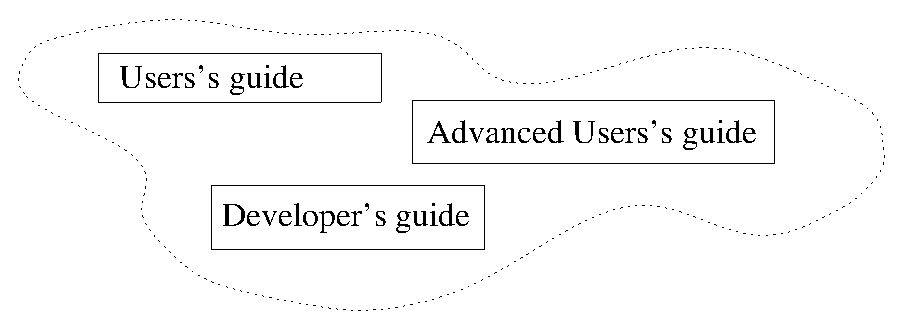
\includegraphics{docstruct.eps}
    \caption{Document Structure}
    \label{fig:docstr}
  \end{center}
\end{figure}

% This document is a User part of two parts of Anick-in-BERGMAN documentation.
% For the second part for internal usage, please, contact J\"orgen Backelin
% directly ({\tt joeb@matematik.su.se})

\section{User's Guide}

This section is dedicated for the users who are interested only in
calculation of Betti numbers.

\subsection{Anick resolution and Betti numbers}

Anick resolution and Betti numbers for the trivial module
are computed for non-commutative
case. (Resolution and Betti numbers for arbitrary module over
non-commutative ring are under development now).

% \begin{tabular}{l | l}  \hline
% Keywords & Description \\ \hline
% -port=\emph{TCP/IP port number}  & tells which port to capture\\
% -help  & tells to print help and exit\\
% -debug  & invokes single thread mode for testing the communication protocol\\
%  \hline
% \end{tabular}\par \noindent

After entering BERGMAN (see the original documentation ``Bergman 1.0 User
Manual'') one will have to perform the following minimal set of commands
in order to have the result calculated:
\begin{enumerate}
\item {\bf (noncommify)}\\
	switchs on to the non-commutative mode;
\item {\bf (load anick)}\\
	load the corresponding binary file for Anick resolution;
\item \label {it:bettiflag} {\bf (onflybetti t)}\\
	sets the option for calculating betti numbers. Instead of
	{\bf (onflybetti t)} it is possible to use {\bf (calcbetti t)}
	in which case the system will not print Betti numbers after
	each degree Gr\"obner basis was calculated;
\item {\bf (setmaxdeg degree)}\\
	limits the process with some  maximal degree;
\item {\bf (simple)}\\
	tasking up the date for Gr\"obner basis calculation as
	described in ``Bergman 1.0 User Manual'';
\item {\bf (calculateanickresolutiontolimit maxdeg)}\\
	invokes the method for calculation of the Anick resolution till the
	specified degree. All the intermediate results, if any,  are printed
	on the terminal.
\item {\bf (anickdisplay)}\\
	prints the result resolution into the file which name is assigned
	to the variable {\bf Anickresolutionoutputfile}. If no file name
	is assigned the result by default will be printed in the file
	{\bf andifres.txt}
\end{enumerate}

% Two following flags should be switched on:
% \begin{itemize}
% \item {\bf (on calcbetti)} -- turns on the Betti numbers
%   calculation  mode.
% \item {\bf (on onflybetti)} -- informs the application to calculate Betti
%  numbers after each degree of Gr\"{o}bner basis is operated out.
%  This allows to view Betti numbers degree by degree  during the
%  Gr\"{o}bner basis computations.
% \end{itemize}


%anDIFFTIME - time in milliseconds taken by processor
%for  operations related computing resolution elements
%(differentials).

% anBETTITIME - time in milliseconds taken by processor
%for  operations related computing Betti numbers.

The item \ref{it:bettiflag} is optional and can be skiped if there is no need
to calculate Betti numbers.
Let us see an example of Anick resolution and Betti numbers
computation:

\begin{verbatim}

1 lisp> (NONCOMMIFY)
nil
2 lisp> (LOAD anick)
nil
3 lisp> (SETQ MAXDEG 4)
4
4 lisp> (ONFLYBETTI T)
nil
6 lisp>  (SETQ ANICKRESOLUTIONOUTPUTFILE "resolution.txt")
"resolution.txt"
7 lisp> (SIMPLE)
Now input in-variables and ideal generators in algebraic form, thus:
        vars v1, ..., vn;
        r1, ..., rm;
where v1, ..., vn are the variables, and r1, ..., rm the generators.
algebraic form (noncomm.) input> vars x,y;
algebraic form (noncomm.) input> x*y;
Anick's resolution initialization...
B(1,1)=2
Anick's resolution initialization done.
+t^2*(z^2)
% 2
x*y,

Calculating Anick's resolution in degree 2...
B(1,1)=2
B(2,2)=1
    0   1   2
  +----------
0 | 1   2   1
1 | -   -
end of Calculations.
Done
 - All is OK (I hope). Now you may (e. g.):
   - kill bergman with (QUIT); or
   - interrupt bergman with ^Z; or
   - clear the memory with (CLEARALL), and run a new (SIMPLE).
nil
8 lisp>  (CALCULATEANICKRESOLUTIONTOLIMIT MAXDEG)
Calculating Anick's resolution in degree 3...
B(1,1)=2
B(2,2)=1
    0   1   2
  +----------
0 | 1   2   1
1 | -   -
end of Calculations.
Calculating Anick's resolution in degree 4...
B(1,1)=2
B(2,2)=1
    0   1   2
  +----------
0 | 1   2   1
1 | -   -
end of Calculations.
nil
9 lisp> (ANICKDISPLAY)

7
10 lisp>

\end{verbatim}

The example should be more or less clear except the last result --
the digit 7 obtained after {\bf (anickdisplay).}  It is related to the
Lisp conception of channel oriented input/output.
Each channel has a corresponding number, and 7 is the current one
in this example. You can see the computed
resolution in the file {\bf resolution.txt} in your current directory.

For this example it contains just:\par \noindent

\begin{verbatim}
D(1, xy)=x.y
B(1,1)=2
B(2,2)=1
    0   1   2
  +----------
0 | 1   2   1
1 | -   -

\end{verbatim}

D(1, xy)=x.y  means that there exists the only 1-chain -- $xy$ and the
differential $d_1$ acts as
$$ d_1: xy\otimes 1 \rightarrow x\otimes y.$$
(see more comments about the Anick resolution for example in
V.Ufnarovski, ``Introduction to Noncomutative Gr\"{o}bner Bases
Theory'',
in ``Gr\"{o}bner Bases and Applications'', Lect.Notes. London
Math.Soc, 251, 1998, Cambridge Univ. Press).

\section{Procedures description}
\subsection{Type Convention}
 Now we describe all the functions
 and their arguments used in the Anick module. Every function
 description has the following structure:
\begin{center}
   \mbox{FUNCTION (ARG$_1$:TYPE$_1$, ARG$_2$:TYPE$_2$, ..., ARG$_n$:TYPE$_n$)
 : RESULT ; COMMENT}
\end{center}
 where ARG$_i$ are identifiers and TYPE$_i$ are their types (see Table
 \ref{typetable}). Then the description of each argument and of the
 result follows. The COMMENT part is explained in {\tt "types.txt"} in the
 bergman doc directory. The following types are used:
\begin{center}
\label{typetable}
\begin{tabular}{l | l}  \hline
{\bf Abbreviation} & {\bf Description}\\ \hline
     id                  &  Identifier\\
     coeff  (non-zero)   &  Coefficient (not necessary an integer)\\
     chn                 &  Chain\\
     qpol                &  quotient polynomial\\
     inputmatrix         &  Matrix of coefficients (in proper input form)\\
     matrix		 &  Matrix of coefficients in internal bergman\\
			 &  form. (Actually a sub-type of llgenredandcoeff)\\
     int                 &  Integer\\
     btnum               &  Betti number\\
     augmon              &  Augmented Monomial\\
     -                   &  Void (No or arbitrary return, not to be used)\\
     bool                &  NIL or non-NIL\\
     any                 &  Any Structure\\
     zero                &  Internal Representation of Zero\\
     ---&\\
     l@@@                &  Prefix "l" stands for: "list of @@@"\\
     (a@@ . b@@)         &  Dotted pairs of objects of types a@@ and b@@.\\
     dl@@@ := (int . l@@@) &  Degree list. \\
     dp@@@               &  Prefix "dp" stands for: "dotted pair (@@@ . @@@)"\\
                         &  (For more information about prefixes and other\\
			 &  types, see "types.txt" in the bergman doc\\
                         &  directory).\\ \hline
\end{tabular}\par \noindent
\mbox{Table \ref{typetable}: Type Convention}
\end{center}

\subsection{Mode settings}


% \subsection{Advanced User's Guide}
\subsection{List of functions for an advanced user}
\begin{description}
\item[MEMBER2NIL (element:any, list:lany) : genint ; DESTRUCTIVE (2)] \mbox{} \\
	Searches list for its first occurrence of element.
	If found, the occurrence is (destructively) replaced by
	NIL, and the number of the position of element in list is
	returned. If element is not found in list, NIL is returned.
\item[PRINTBETTINUMBER (btnumber:btnum) : - ;] \mbox{} \\
	Prints Betti number btnumber as follows: B(order, degree) = value.
\item[GETBETTINUMS () : lbtnum;] \mbox{} \\
	Returns the list of Betti numbers.
\item[GETBTORDER (btnumber:btnum) : int ;] \mbox{} \\
        Returns the order of Betti number btnumber.
\item[GETBTDEGREE (btnumber:btnum) : int ;] \mbox{} \\
        Returns the degree of Betti number btnumber.
\item[GETBTVALUE (btnumber:btnum) : int ;] \mbox{} \\
        Returns the value of Betti number btnumber.
\item[PRINTBETTI () : - ;] \mbox{} \\
	Prints all the calculated  Betti numbers.
\item[PRINTCURRENTBETTI () : - ;] \mbox{} \\
	Prints Betti numbers for the last calculated Gr\"obner basis
	degree.
\item[CLEARRESOLUTION () : - ;] \mbox{} \\
	Clears all the corresponding variables and streams for the
	resolution.
\item[PRINTCHAIN (chain:chn) : - ;] \mbox{} \\
	Prints chain. The vertices are printed as monomials
	(corresponding to the present ALGOUTMODE and minor output
	mode settings). If PRINTEDGESTRING is ON, then between
	vertices it prints the value of anEDGESTRING.
\item[MPRINT (mat:matrix) : bool ;] \mbox{} \\
	Prints mat as a matrix to standard output and returns T, if
	that is not NIL. Else it prints nothing and returns NIL.
\item[CFLINEPRINT (ln:lcoeff) : bool ;] \mbox{} \\
	Prints the list of coefficients ln in one line and returns
	T if ln is non-NIL. Else it prints nothing and returns NIL.
\item[RANK (mat:inputmatrix) : int ; DESTRUCTIVE] \mbox{} \\
	Returns the rank of mat calculated in present coefficient
	field.
\item[INPUTMATRIX2REDANDMATRIX (mtrx:inputmatrix) : matrix ; DESTRUCTIVE] \mbox{} \\
	Modifies the elements of mtrx so that their type is of
	acceptance by further procedures.
\item[PRETTYPRINTSDP (pol:tp) : - ;] \mbox{} \\
	Prints the semi-distributed polynomial pol in a form decided by
	the tensor polynomials print-mode. (See GETTENSORPOLSPRINTMODE).
\item[PRINTTENSORPOLSDISTRIBUTED () : - ;] \mbox{} \\
	Selects distributed form for printing semi-distributed
	polynomials.
\item[PRINTTENSORPOLSSEMIDISTRIBUTED () : - ;] \mbox{} \\
	Selects semi-distributed form for printing semi-distributed
	polynomials.
\item[GETTENSORPOLSPRINTMODE ()  : id ;] \mbox{} \\
        Returns the identifier which is a keyword either DISTRIBUTED
	or SEMIDISTRIBUTED. This identifier points out how the current
	semi-distributed polynomials are printed.
\end{description}

% \section{Developer's Guide}
\subsection{The description of further procedures for developers}
\begin{description}
\item[SETTENSPOLPRTSTRINGS (strings:lstr) : lstr ;] \mbox{} \\
        The list strings should consist of 3 strings which are
	used to print tensor product. First string is printed
	at the beginning, second - as a tensor multiplication sign
	and the third - as the ending of thensor monomial.
	The list of 3 strings of old settings is returned.
\item[GETTENSPOLPRTSTRINGS () : lstr ;] \mbox{} \\
	Returns a list of 3 strings which are used when tensor
	monomials are printed as beginning, middle and ending
	strings.
\item[SETEDGESTRING (strng:string) : genstring ;] \mbox{} \\
        The string strng is taken for printing as edges when chain
	vertexes are printed. The old value of it is returned.
\item[GETEDGESTRING () : - ;] \mbox{} \\
        Returns the value of string which is printed between chain
	vertexes.
\item[PRINTNEWCHAINSDIFF (chan:genint) : - ;] \mbox{} \\
        Prints differentials for the new generated chains
	to the channel chan
\item[PRINTCHAINSDIFF (chan:genint) : - ;] \mbox{} \\
        Prints differentials for the all generated chains
	to the channel chan
\item[PRINTCHNDIFF (inchain:chn) : - ;] \mbox{} \\
        Prints differential for the chain inchain in form
        D (chain length, chain) = differential
\item[anBETTIINIT () : - ;] \mbox{} \\
	This procedure initializes variables which are used to collect
	information about Betti Numbers. It should be called before
        Anick calculation.
\item[anbtNUMBEROFCHAINS (degree:int, chains:dlchn) : int ;] \mbox{} \\
	This function accepts a homological degree of a chain,
	a degree list for all chains, and returns the number of chains
	of that degree in that list.
\item[anbtZEROPROLONG (tail:lratcoeff, n:int) : lcoeff ;] \mbox{} \\
	Returns a list whose first n elements are NIL (representing
	the coefficient zero), and which than continues with the list
	``tail''.
\item[anBETTI(chains:(int . lchn)) : - ;] \mbox{} \\
	The procedure accepts as its argument a list which is an
	element of the anCHAINS degree list. The procedure
	updates Betti numbers which are storied in anCURRENTBETTINUMS.
\item[anALLBETTI () : - ;] \mbox{} \\
	This procedure applies the procedure anBETTI to all elements
	of the anCHAINS list. It should be called if the calculation
	of Betti numbers was not invoked during calculation of the Groebner
	basis.
\item[ResolutionInit () : - ;] \mbox{} \\
	This procedure initializes all the variables concerned with
	the Anick resolution. It needs information about Groebner
	basis generators, therefore, it should be called after the
	system has them.
\item[anifResolutionFixDegree (dgr:int) : - ;] \mbox{} \\
	For a given degree it calculates chains and the Anick
	resolution differentials, and prints them into the result
	file. It also updates related variables.
\item[ResolutionFixcDegEnd () : - ;] \mbox{} \\
	Applies the procedure anifResolutionFixDegree for 
	all the degrees which has to be fixed in anifResolutionFixDegree
	sense.
\item[ResolutionDone() : - ;] \mbox{} \\
	Closes the output stream used in Anick related procedures.
\item[ResolutionClear () : - ;] \mbox{} \\
	Cleans up all the Anick related variables including Betti
	numbers.
\item[anPROLONGCHAIN (inchain:chn, intail:augmon) : (chn . augmon) ;] \mbox{} \\
	inchain should be an n-chain and intail an augmon, such that
	there is an (n+1)-chain "outchain" which is a left factor
	of inchain * intail. Then (outchain . outtail) is returned,
	where outtail fulfills
        inchain * intail� = outchain * outtail.
	(Else, an error may be signaled, or the result may be
	arbitrary.)
\item[anCONSTRUCTNEWCHAINS (inchain:chn, degdiff:int) : - ;] \mbox{} \\
	Constructing new chains from inchain and a total
	degree difference number degdiff. The new chains
	represent the chains of length = 1 + length[inchain] and
	total-degree = degdiff + totaldegree[inchain], and with
	inchain as a left factor. They are sorted into their
	proper positions on anNEWCHAINS.
\item[anCONSTRUCTZEROCHAINS () : - ;] \mbox{} \\
	This routine should be called before the calculation of
        Anick's resolution to construct initial data for
        differential and integral recursive functions.
\item[anNEWGBELM2CHAIN (gbelm:augmon) : chn ;] \mbox{} \\
	Returns a 1-chain corresponding to gbelm (which ordinarily
	would be a leading monomial of a new Groebner basis).
	Calculates and sets the differential of the output chain.
\item[anLESSCHAIN (chain1:chn, chain2:chn) : bool ;] \mbox{} \\
	Returns NIL if chain1 doesn't precede chain2 in "monomial
	deg-lex" order.
\item[anDIFF (inchain:chn) : tp ;] \mbox{} \\
	The chain inchain is processed according to the
	algorithm of calculating the differential in the Anick
	resolution. The result semi-distributed polynomial is
	returned.
\item[andiINTEG (pol:tp) : tp ; DESTRUCTIVE] \mbox{} \\
	This procedure is used in the calculation of Anick differential
	in order to complete the algorithm for calculating the Anick
	differential.
\item[anRANK (mat:inputmatrix) : int ; DESTRUCTIVE] \mbox{} \\
	Calculates the rank of mat. It also transforms mat to a
	proper elements type by \\ INPUTMATRIX2REDANDMATRIX procedure.
\item[anCONCATTENSPOLMON (pol:tp, mon:augmon) : tp ;] \mbox{} \\
	Concatenates mon to each element of the tensor polynomial pol
	to the right side, reduces them by means of the current
	Groebner basis, and returns the result.
\item[anMAKETENSPOL (inchain:chn, mon:augmon) : tp ;] \mbox{} \\
	Creates and returns the tensor polynomial which contains only
	one element: inchain tensor multiplied by mon.
\item[anDESTRUCTADDTENSPOLS (pol1:tp, pol2:tp, cf:coeff):tp; DESTRUCTIVE(1)] \mbox{} \\
	Modifies pol1 so that pol1 = pol1+cf*pol2.
	Returns the modified pol1.
\item[anEXTRACTHIGHTENSMON (pol:tp) : (chn . augmon) ;] \mbox{} \\
	Returns a dotted pair which represents a highest
	element in the deg-lex sense of pol.
\item[antpPRINTQPOLORCONSTANT (pol:qpol) : - ;] \mbox{} \\
        Prints a rational coefficient cf, a *, and then within
	parentheses the polynomial multiplied by the inverse of cf.
	If the polynomial is constant, prints only it as a
	rational coefficient.
\end{description}
